\chapter{自动选路系统}
\label{chapter:switching}

针对~\ref{chapter:introduction}章中介绍的应用场景,即在不同地点接收多路短波语音信号,然后再根据质量进行选路的应用场景,本文基于~\ref{chapter:algorithms}章介绍的客观质量评价算法,实现了一个不需要人工参与的短波语音自动选路系统。主要包括多路语音时间对齐算法、选路切换策略等工作,以下分别进行介绍。

\section{两路语音时间对齐}\label{section:align2}

两路语音对齐算法是多路语音对齐算法的基础,这里介绍一种基于互相关的朴素算法。设原始语音为$x(t)$,收到的两路语音信号分别为$y_1(t)$和$y_2(t)$,设两路信号延迟分别为$\delta_1$和$\delta_2$,则有以下关系:
\begin{equation}
\left\{
    \begin{array}{l}
        y_1(t) = x(t-\delta_1) + e_1(t-\delta_1) \\
        y_2(t) = x(t-\delta_2) + e_2(t-\delta_2)
    \end{array}
\right.
\end{equation}

其中$e_1$和$e_2$为两路信号传播过程中分别引入的噪音信号。

选取两路信号开头一定长时间$T,T>>\delta$,计算互相关函数:
\begin{equation}\label{eq:corr}
\begin{array}{c}
    C_{12}(\delta)  = \left\{
    \begin{array}{rcl}
        \int_\delta^Ty_1(t)y_2(t-\delta)dt, && {\delta \geq 0} \\
        \int_0^{T+\delta}y_1(t)y_2(t-\delta)dt, && {\delta < 0}
    \end{array}
    \right. \\
    = \left\{
    \begin{array}{rcl}
        \int_\delta^Tx(t-\delta_1)x(t-\delta_2-\delta)dt+\int_\delta^Te_1(t-\delta_1)e_2(t-\delta_2-\delta)dt, && {\delta \geq 0} \\
        \int_0^{T+\delta}x(t-\delta_1)x(t-\delta_2-\delta)dt+\int_0^{T+\delta}e_1(t-\delta_1)e_2(t-\delta_2-\delta)dt, && {\delta < 0} \\
    \end{array}
    \right.
\end{array}
\end{equation}

上式右边前一部分,在$\delta=\delta_1-\delta_2$时取得极大值,第二部分,假设噪音均为高斯白噪音,则其大小基本不随$\delta$变化。

从而当$\delta=\delta_1-\delta_2$时$C_{12}(\delta)$取得极大值,即:
\begin{equation}
\delta1 - \delta2 = \arg \max C_{12}(\delta)
\end{equation}
记$\delta_{12}=\delta_1-\delta_2$,为$y_1 (t)$相对于$y_2 (t)$的延迟大小,$\delta_{12}>0$表明$y_1(t)$落后于$y_2(t)$,$\delta_{12}<0$表明$y_1(t)$超前于$y_2(t)$。
通过$C_{12}(\delta)$极值点估计出$\delta_{12}$之后,即可通过截取平移获得对齐的两路语音信号$y_1^*(t)$和$y_2^*(t)$:
\begin{equation}
% \left\{
    \begin{array}{l}
        y_1^*(t)=  \left\{ 
            \begin{array}{rcl}
            y_1(t), && {\delta_{12} \geq 0} \\
            y_1(t-\delta_{12}), && {\delta_{12} < 0}
            \end{array}
        \right. \\
        \\
        y_2^*(t)= \left\{ 
            \begin{array}{rcl}
            y_2(t), && {\delta_{12} \leq 0} \\
            y_2(t+\delta_{12}), && {\delta_{12} > 0}
            \end{array}
        \right.
    \end{array}
% \right.
\end{equation}
上述对于相对延时$δ_{12}$的估计受到以下几方面影响会存在一定误差:
\begin{enumerate}
\item 噪音污染可能不是理想白噪音,当噪音污染程度较大时会导致估计误差较大。
\item 两路语音相对延时可能较大,当延迟大小接近$T$的数量级时,截取的信号重叠部分较小,会导致估计误差较大。
\end{enumerate}


\section{多路语音时间对齐} \label{section:align-multi}

在两路语音对齐算法的基础上,本节介绍一种实现多路语音时间对齐的算法。

设收到有$K$路语音$(K\geq3$),分别为$y_1(t), y_2(t), ..., y_K(t)$,设指标集$I={i│i\in N^+, i\leq K}$。首先使用~\ref{section:align2}节的方法我们可以估计出多路语音两两之间的相对延时$\delta_{ij}  (i,j\in I,i\neq j)$。
假设我们的估计不存在误差,且定义$\delta_{ii}=0,(i \in I)$,则
\begin{equation}\label{eq:delay-relations}
\delta_{ij}=\delta_{ik}+\delta_{jk}, \forall i,j,k \in I
\end{equation}

但是由于噪音的存在,延时的估计可能存在误差,所以两两之间的相对延时会存在不一致的情况,即公式~\ref{eq:delay-relations}并不恒成立。因而就需要从所有$K(K+1)/2$个相对延时中选取$K-1$个以确定一个统一的一致的,各路语音的相对延时。

一种最简单朴素的方法是以某一通道语音为基准,直接选取所有其他通道语音和该路语音的相对延时。例如以$y_1 (t)$为基准,选取$\delta_{1i}  (i \in I, i \neq 1)$作为统一标准确定各路语音的延时。但是这种方法得出的结果未必是最优的,如果 $y_1 (t)$ 受到的噪音污染较大,则很有可能得出的结果误差相当大。对此问题可以考虑使用后面介绍的语音质量客观评价方法来选取一路质量最优的语音作为参考基准。但是即便如此依然存在问题:如果选取的基准路语音$y_k (t)$和其他几路语音相对延时较大,而其他几路语音之间的相对延时较小,则估计的$y_k (t)$和其他几路语音的相对延时也会有较大误差,不如选取其他几路语音之间的相对延时加上$y_k (t)$和某一路语音的相对延时更好。

针对以上讨论的问题,以下介绍一种基于图论最小生成树算法来选取相对延时的方法。

我们的目标是要选取$K-1$个相对延时将所有K路语音关联起来,并使得选取的相对延时是估计准确性尽量高的。根据~\ref{section:align2}节的分析,对两路语音之间相对延时的估计的准确度可以通过互相关峰值的大小来反应,互相关的峰值越大,则准确性越高。以各路语音为节点构建一个全连通的有权无向图,各边的权值设为相连节点代表的两路语音之间互相关峰值的大小,则我们的目标可以描述为:选取$K-1$条边将$K$个节点连成一颗树,并使得$K-1$条边的权值和在所有的生成树中最大。即构造如下有权无向图
\begin{equation}
\begin{array}{l}
G(V,E), \\
V = I, \\
E = \left\{(i,j)|i, j\in I, i \neq j\right\}, \\
w(i,j)=\max⁡ \left\{ C_{ij}(\delta) \right\}
\end{array}
\end{equation}

问题即转化成求解图$G$的最大生成树,最大生成树和最小生成树可互相转化,直接对所有边权重求相反数即可。

求解最小生成树问题的经典算法有Boruvka算法、Prim算法和Kruskal算法等。Boruvka算法是最古老的最小生成树算法,时间复杂度为$O(|E|log|V|)$;Prim算法和Kruskal算法是最常用和广为人知的两种最小生成树算法,时间复杂度分别为$O(|E|+|V|log|V|)$和$O(|E|log|E|)$。Yao~\cite{YAO197521}在Boruvka算法基础上改进提出了一种更快速的算法,时间复杂度为$O(|E|loglog|V|)$。而Karger等人~\cite{Karger:1995:RLA:201019.201022}提出的线性时间算法是目前最快的最小生成树算法。

得到最大生成树后,生成树上对应的边即代表应该选取的相对延迟估计,在这$K-1$个相对延迟的基础上,利用式x.x.x即可求出各路信号相对$y_1 (t)$的延迟$\delta_{i1},(i \in I)$,其中$\delta_{11}=0$。随后对各路信号进行对齐和平移,得到时间对齐后的信号:
\begin{equation}
y_i^* (t)=y_i (t+\delta_{i1}-\min_{j\in I}\delta_{j1})
\end{equation}

\section{实时多路对齐算法} \label{section:realtime-align}

\begin{figure}
\centering
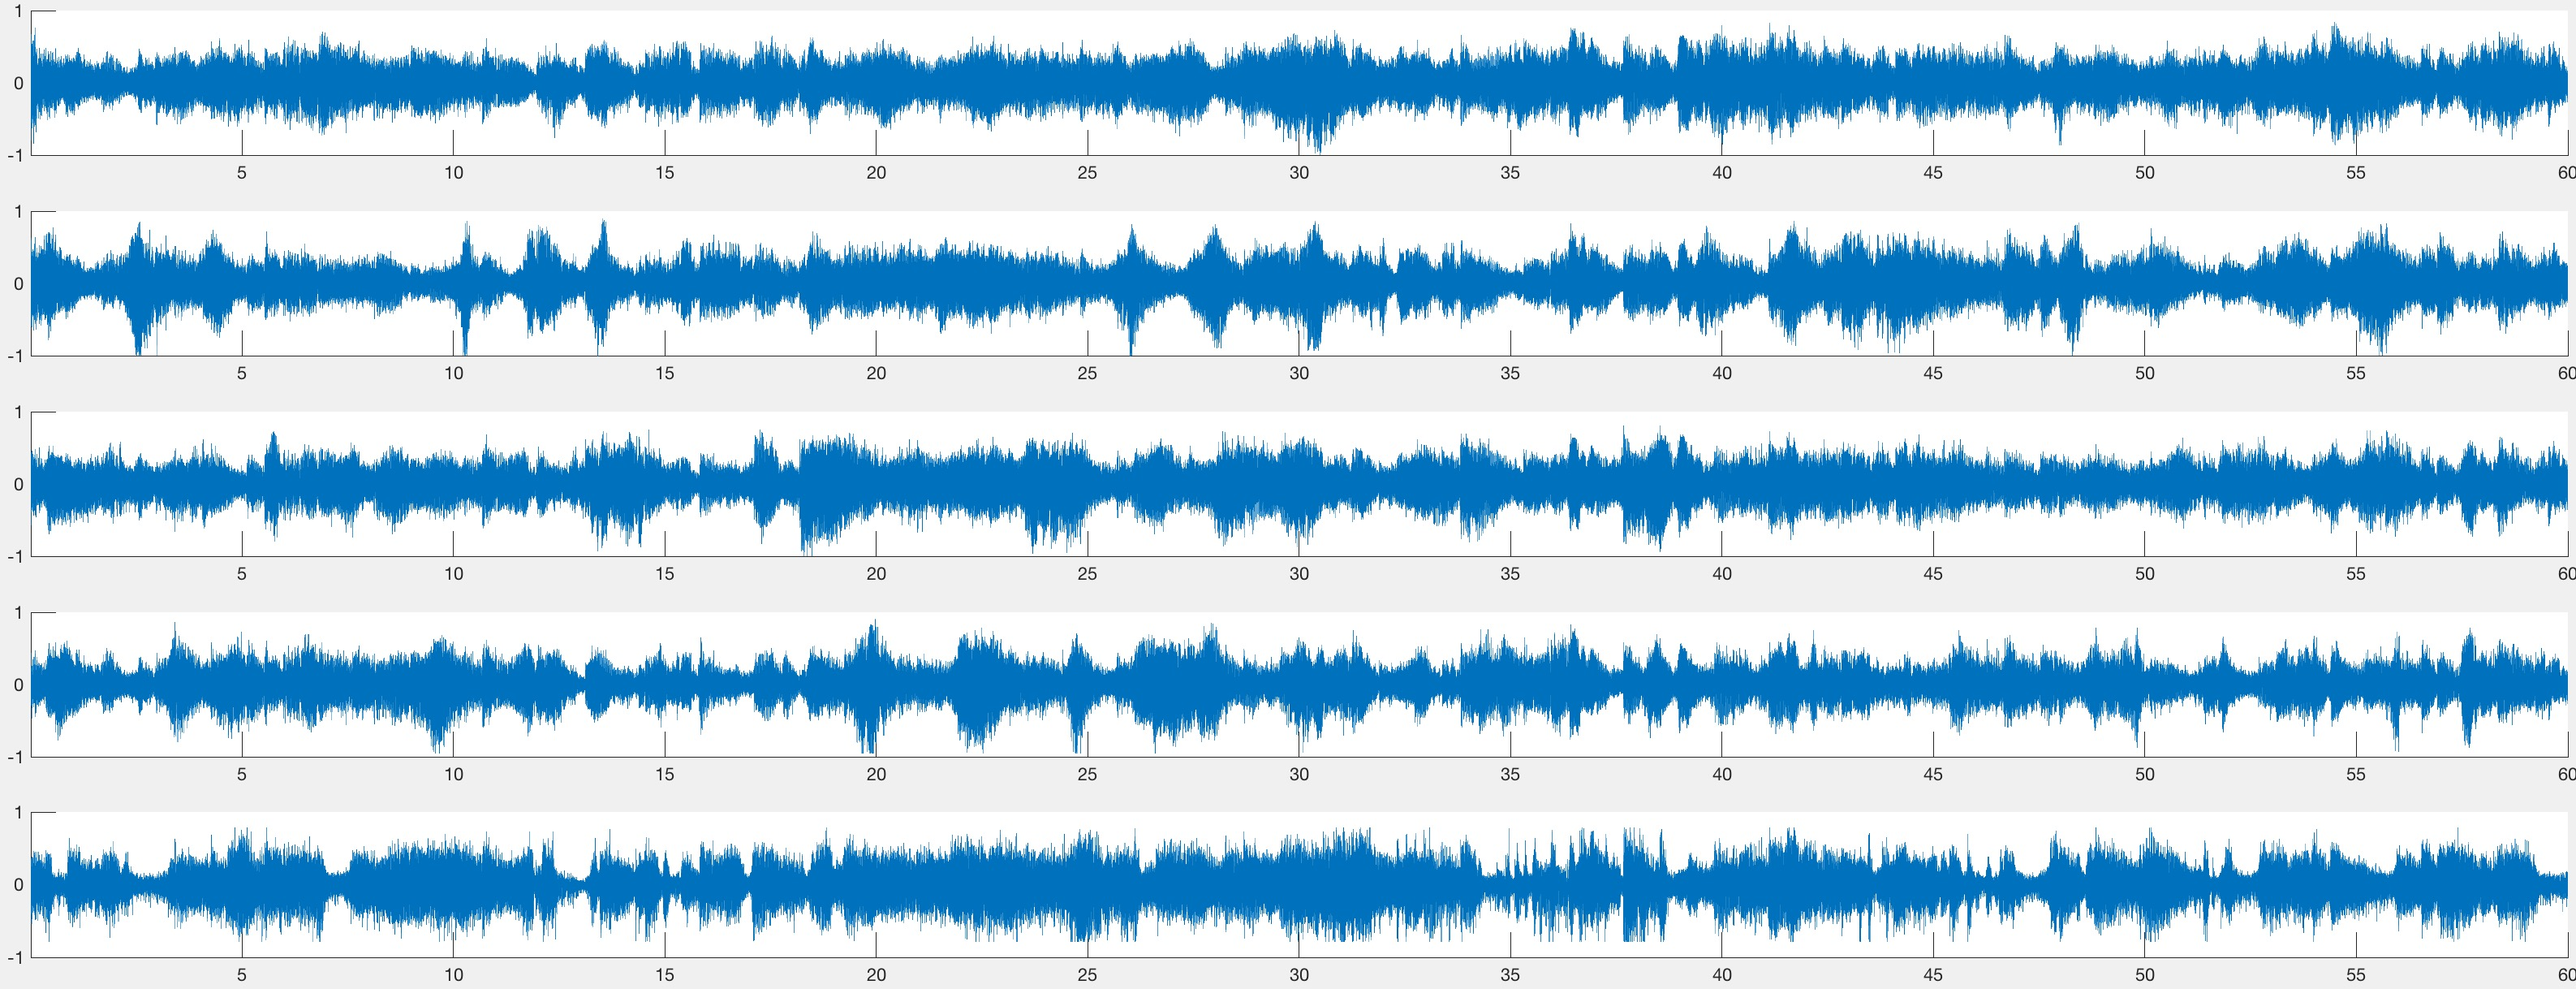
\includegraphics[width=0.8\textwidth]{multi-align}
\caption{实时对齐算法示意\label{fig:multi-align}}
\end{figure}

实际应用中,往往要求对多路语音信号进行实时处理。在~\ref{section:align-multi}节基础上,本节介绍一种对于多路语音信号流进行实时对齐的算法。

首先对于每一路语音使用一个缓冲队列存储最近一段时间的信号,新来的信号从队尾加入队列,而随着时间推移,队首信号不断出队列,本算法通过控制各路信号出队列的时间,使得从队首出队的信号是时间对齐的。

如图~\ref{fig:multi-align}所示,为方便描述,可以将离散语音信号想象成一个无限长的队列,然后有一个队首指针和队尾指针,两个指针之间的部分即使算法目前实际缓存的语音信号部分。由于随着时间推移不断接收到新的信号,所以队尾指针会随着时间以固定速率后移,而队首指针则是在算法控制下后移以调整延时,最终稳定时,队首和队尾的指针均匀速后移,各路信号缓存的长度不同,队首指针处的信号是时间上对齐的。

算法一开始首先保证各路信号均缓存了时间长度为的数据。随后使用~\ref{section:align-multi}节中的算法可以得出各路信号相对第一路信号的延迟$\delta_{i1}, i \in I$,可能为负值,找到最大的延时,记为$\delta_{k1} = \max \delta_{i1}$,则为了保证队首指针时间对齐,第$i$路信号的队首指针应暂停$\delta_{k1}-\delta_{i1}$时间不移动。这相当于第$i$路信号的延迟增加了$\delta_{k1}-\delta_{i1}$,于是各路信号的队首均对齐到了路信号。之后每0.1秒执行一次上述步骤进行对齐调整。
进一步,为了保证算法的稳定性,降低执行过程中对于相对延时突发的错误估计造成的影响,可以设置一个调整步长$0<\alpha<1$,各路队首指针暂停时间修改为$\alpha(\delta_{k1}-\delta_{i1})$。$\alpha$越大则越快收敛到对齐状态,但是越不稳定;相反越小则收敛速度越慢,但是越稳定。可以根据情况设定$\alpha$的取值。
另外,此方法永远在增加信号的延迟,会导致合路信号的延迟越来越大,可以做如下改进:每次对齐调整完成后,如果最短的缓存队列长度为超过了$T$,则所有路信号的队首指针同时向后调整使得最短的缓存队列长度缩短为$T$。这样,合路信号的延迟永远为延迟最大的一路信号的延迟加上$T$。

\section{选路策略及系统设计}

本节介绍短波语音信号的选路策略以及选路系统的设计。由于各路信号的强度和背景噪音不同,如果直接对各段时间内的信号,总是切换到质量评分最高的一路信号,可能出现信号切换过于频繁,导致听起来连贯的问题,反而影响合路信号的质量。以下几项策略保证了合路信号在选择尽量优质量的语音通路的同时,提高合路语音的自然度。
\begin{enumerate}
    \item 需要对各路语音的功率进行归一化处理,可以使用各路语音的均值功率作为参考,将各路语音信号放大或缩小从而统一功率。
    \item 为防止意外状况导致的错误评分带来的抖动,对各路语音的实时评分经过一个低通滤波作为选路参考的分值。
    \item 为了避免过度频繁的切换语音通路,设定一个适当大小的阈值,只有当新的最优通路的评分超过当前选择通路的评分达到一定阈值,才切换至新的最优通路。否则依然保持原来选择的通路。 
    \item 在通路切换时,采用线性渐变的过度来平滑切换的过程。
\end{enumerate}

\begin{figure}
\centering
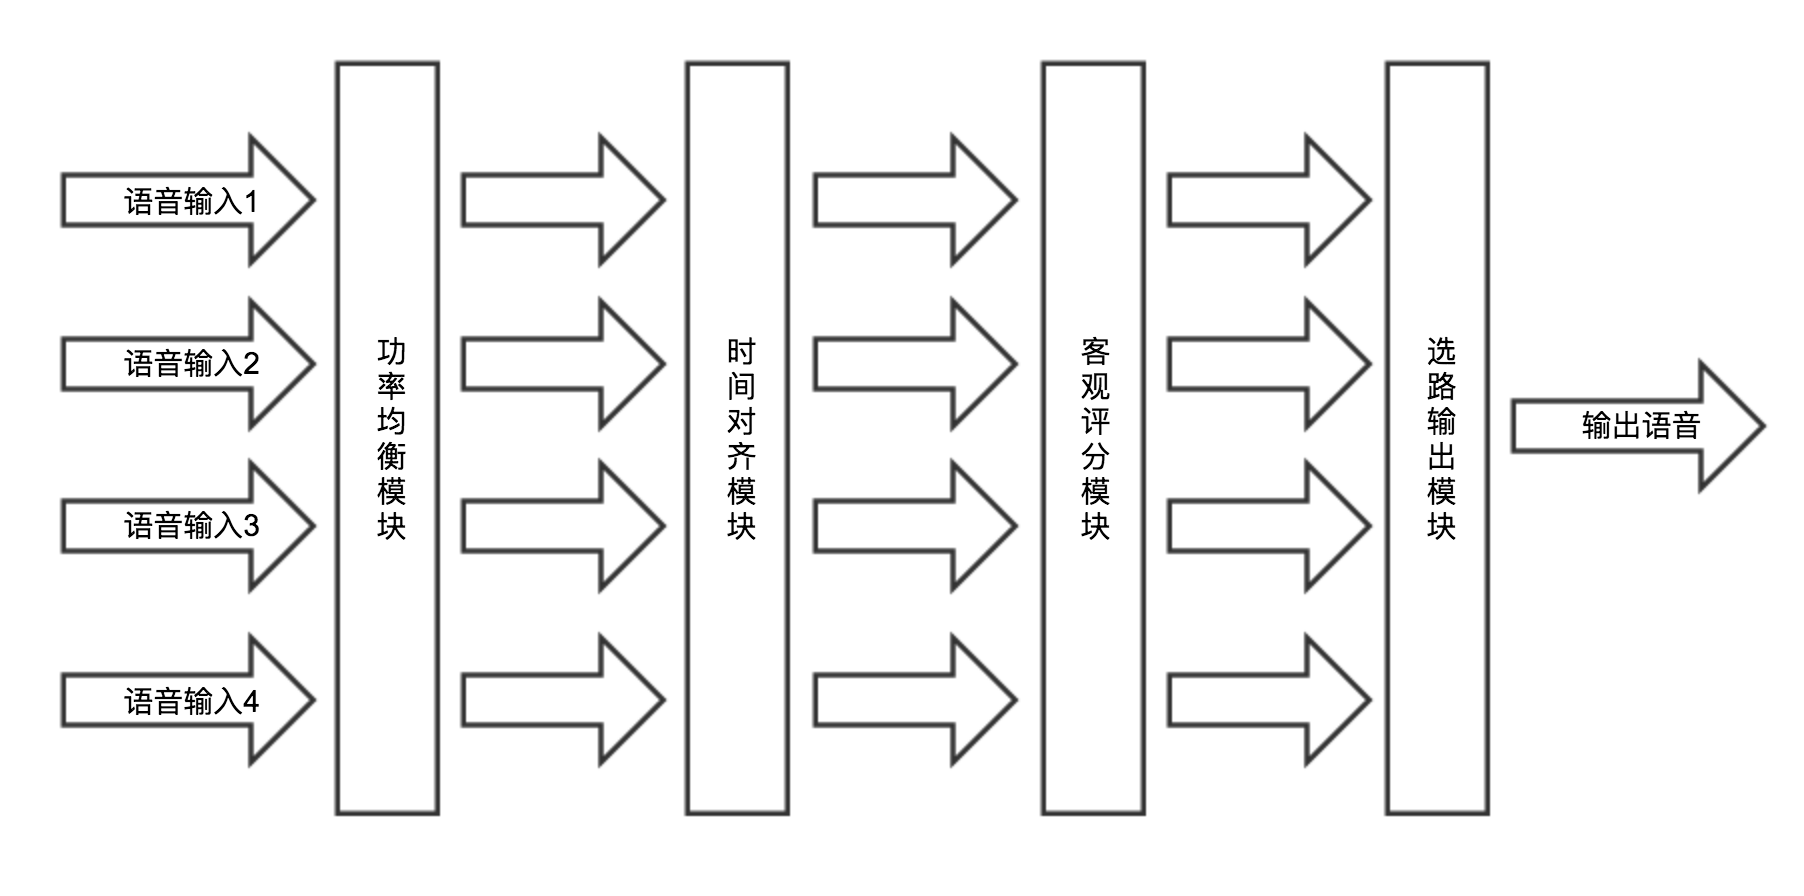
\includegraphics[width=0.8\textwidth]{switching-sys}
\caption{选路系统结构\label{fig:switching-sys}}
\end{figure}

如图~\ref{fig:switching-sys}所示,选路系统分为“功率均衡模块”、“时间对齐模块”、“客观评分模块”、“选路输出模块”这四个模块,分别实现上述几项策略。

功率均衡模块负责均衡各路语音信号的功率,具体步骤如下:统计每一路输入最近1s时间内的信号功率$P_i, i \in I$,将其经过一个低通滤波器,得到滤波后的平均信号功率$\bar{P_i}$,据此可利用式~\ref{eq:power-gain}计算各路的信号增益$Gain_i$,各路信号分别乘上对应增益实现各路信号的功率均衡。
\begin{equation}\label{eq:power-gain}
Gain_i = \sqrt{\frac {K\bar{P_i}} {\sum_{k \in I}{\bar{P_k}}} }
\end{equation}

时间对齐模块负责各路语音信号的时间对齐,利用~\ref{section:realtime-align}节介绍的算法实现。

客观评分模块对每一路最近1s内的信号使用~\ref{chapter:algorithms}章介绍的算法进行客观评分,然后再通过低通滤波器得到去除抖动后的质量评分$\bar{S_i}, i \in I$。

选路输出模块负责选路切换,设定切换阈值$T_{switch}$,若当前输出为$i$路语音,切换到第$j$路语音的条件为:
\begin{equation}
\begin{array}{l}
\bar{S_j} = \max\limits_{k \in I} \bar{S_k} \\
\bar{S_j} - \bar{S_i} > T_{switch}
\end{array}
\end{equation}
在发生切换时,切换模块自动完成线性平滑过度,设定切换时长为$\Delta$,则切换阶段输出语音可表示为:
\begin{equation}
y_{out}(t) = \frac{ty_j(t)+(\Delta-t)y_i(t)}{\Delta}
\end{equation}

\begin{algorithm}
    \caption{自适应的活动台检测算法}
    \label{alg:container_split_adaptive}
\begin{algorithmic}[1]
\INPUT
    \Statex 果蝇行为视频;
    \Statex 活动台的数量$K_1$;
    \Statex 活动台圆的数量$K_2$;
    \Statex 活动台的最大可能半径$R_{max}$ 和 最小可能半径 $R_{min}$;
    \Statex Hough圆检测参数最大自适应次数$max\_iters$。
\OUTPUT
    \Statex 活动台的圆心$(x_1, y_1), \ldots, (x_{K_1},y_{K_1})$;
    \Statex 活动台的外径$R$;
    \Statex 活动台的移入时刻$t_{1, in}, \ldots, t_{K_1, in}$和移出时刻$t_{1, out}, \ldots, t_{K_1, out}$;
\State 从视频中抽取$M_1$帧视频$\{ I_{k_1}, I_{k_2}, \ldots, I_{k_{M_1}} \}$;
\State 初始化Hough圆检测的参数 $param_1^{\{0\}} = 200$, $param_2^{\{0\}} = 200$;
\For {$i = 0$ to $max\_iters$;}
    \State 对视频帧$\{ I_{k_1}, I_{k_2}, \ldots, I_{k_{M_1}} \}$,使用参数$param^{\{i\}}_1$和$param^{\{i\}}_2$进行Hough圆变换检测,得到$N_i$个圆;
    \If {$N_i < 3K_1$; }
        \State $param_1^{\{i+1\}} = 0.9\times param_1^{\{i\}}, param_2^{\{i+1\}} = 0.9\times param_2^{\{i\}}$
    \Else
        \State break
    \EndIf
\EndFor
\State 从视频中抽取$M_2$帧视频$\{ I_{l_1}, I_{l_2}, \ldots, I_{l_{M_2}} \}$
\State 使用参数$param_1 = param_1^{\{i\}}, param_2 = param_2^{\{i\}}$,利用Hough圆检测算法,对视频帧$\{ I_{l_1}, I_{l_2}, \ldots, I_{l_{M_2}} \}$进行圆检测,得到$N$个圆 $(\tilde{x}_1, \tilde{y}_1, r_1), \ldots, (\tilde{x}_N, \tilde{y}_N, r_N)$;
\State 使用GMM算法\cite{GMM_1999}将圆心$(\tilde{x}_1, \tilde{y}_1), \ldots, (\tilde{x}_N, \tilde{y}_N)$聚为$K_1$类,得到$(x_1, y_1), \ldots, (x_{K_1},y_{K_1})$;\label{alg:arena:clusterXY}
\State 使用GMM算法将半径$r_1, \ldots, r_N$聚为$K_2$类,得到$R_1, R_2, \ldots, R_{k_2}$,最终活动台的外径为$R = \max(R_1, R_2, \ldots, R_{k_2})$;\label{alg:arena:clusterR}
\State 检测$(x_i, y_i)$周围检测到的Hough圆的数目,利用二分查找法,分别查找$K_1$个聚类中心的移入视频的时刻$t_{i,in}$和移出视频的时刻$t_{i, out}$;
\State 输出$(x_1, y_1),\ldots,(x_K, y_K)$、$R$和$t_{1, in}, \ldots, t_{K_1, in}$以及移出时刻$t_{1, out}, \ldots, t_{K_1, out}$。
\end{algorithmic}
\end{algorithm}

\section{小结}

本章主要介绍了自动选路系统。
